\documentclass[a4paper,12pt]{article}
\usepackage[MeX]{polski}
\usepackage[utf8]{inputenc}
\usepackage{graphicx}
%opening
\title{Dama z Auxerre}
\author{Dawid Laskowski}



\begin{document}
\maketitle 
 \emph{Dama z Auxerre} --- przedstawiająca postać kobiecą grecka rzeźba z okresu archaicznego, znajdująca się obecnie w zbiorach Luwru.

Wykonana z~ wapienia figurka ma zaledwie 75 cm wysokości[1][2]. Datowana jest na 2. połowę VII wieku p.n.e. Przedstawia postać żeńską w~pozycji frontalnej, ze złączonymi nogami. Kobieta ubrana jest w~ okrywający szczelnie jej ciało peplos, z~ pasem oddzielającym wyraźnie tors od dolnej części ciała. Prawą rękę trzyma złożoną na piersi, lewa natomiast opuszczona jest wzdłuż ciała. Głowa od góry jest spłaszczona, zdobią ją loki opadające na ramiona (po 4 z każdej strony) i~na plecy .~~Twarz ma trójkątny zarys, wargi postaci są nieco uniesione ku górze, przypominając późniejszy archaiczny uśmiech. Czoło jest niskie, oczy zaś mają migdałowaty kształt. Szata zdobiona jest ornamentem w~ postaci kwadratów wpisanych jeden w drugi.Spod szaty wystają gołe stopy, spoczywające na czworokątnej bazie wykutej wraz z~ posągiem z jednego bloku[3]. Przypuszcza się, że figurka może być przedstawieniem jakiejś bogini.

Rzeźba pochodzi przypuszczalnie z Krety. Jej dzieje są nieznane; w 1895 roku została nabyta na aukcji za jednego franka przez Louisa Davida, woźnego teatru miejskiego w Auxerre, od paryskiego rzeźbiarza nazwiskiem Bourgoin. Przez kilka lat stanowiła ozdobę teatru, w 1908 roku została przeniesiona do miejskiego muzeum.Tam została zauważona przez kuratora muzeum w Luwrze Maxime’a Collignona, który zabrał ją ze sobą do Paryża.

\section{Przypisy}\label{sec:tekst}
\subsection{}\label{sec:tekst} \emph{Encyclopedia of the History of Classical Archaeology.}~ edited by Nancy Thomson de Grummond. London: Routledge, 1996, s.~110-111.~ISBN 1-884964-80-X.
\subsection{}\label{sec:tekst} 
 Fred Kleiner: Gardner’s Art Through the Ages. \emph {A Global History}. Wyd.~13. Boston: Wadsworth, 2009, s. 105. ISBN 978-0-495-09307-7.
\subsection{}\label{sec:tekst} 
Alfred Twardecki: \emph {Mały słownik sztuki starożytnej Grecji i Rzymu}.Warszawa: Unia wydawnicza Verum, 1998. ISBN 83-85921-75-3.

\emph{Linki zewnętrzne}
Opis zabytku na stronie internetowej Luwru
\emph{Soliści}
\begin{table}[h]
\begin{tabular}{clc}
\hline
\textbf{Pozycja}&\textbf{Zawodnicy}&\textbf{Punkty}\\
\hline
1&Iwan Pawłow{,}&221.07{,}1\\
2&Irakli Maisuradze{,}&200.73{.}1\\
3&Larry Loupolover{,}&195.09{,}1\\
4&Murad Kurbanow{,}&193.07{,}1\\
5&Nicholas Vrdoijak{,}&191.73{.}1\\
6&Jegor Muraszow{,}&195.09{,}1\\
7&Lee June {,}&190.73{.}1\\
8&Marcus Bjork{,}&167.09{,}1\\
9&Jewgienij Własow{,}&150.07{,}1\\
10&Nicky Leo Obrejkow{,}&160.73{.}1\\
11&Aliaksej Miałiochin{,}&140.09{,}1\\
\hline
\end{tabular}
\caption{osiągnięcia}
\end{table}

\emph{Korczówka} --- wieś sołecka w Polsce położona w~województwie lubelskim, w~powiecie bialskim, w~gminie Łomazy.

Miejscowość jest siedzibą rzymskokatolickiej parafii Parafia św.~Jozafata.

W latach \empt{ 1975–1998}~miejscowość administracyjnie należała do województwa bialskopodlaskiego.


Historia

\emph  {Korczówka} w wieku XIX opisana jako: wieś i folwark w powiecie bialskim, gminie Lubenka, parafii katolickiej Łomazy. We wsi cerkiew parafialna dla ludności rusińskiej.
W r. 1827~było tu 22~domów i 125~mieszkańców. W 1883~spisano 26~domów i 172~mieszkańców.

Dobra Korczówka składają się z folwarku: Korczówka i osady Rososz (Roskosz, dawniej Rozkosz, Rososz), wsi Korczówka, Wólki Korczowskiej i wsi Burwin. Rozległość folwarczna wynosiła 1141~mórg w tym: grunta orne i ogrody 400~mórg, łąk było 237~mórg, pastwisk mórg 79. Las stanowił 390~mórg, nieużytki i~place 35~mórg. Folwark posiadał budynków murowanych 7, drewnianych 15. W okolicy pokłady torfu.

Osada Rososz posiadała osad 361, z~ gruntem 8998~mórg. Wieś Korczówka osad 23, z~ gruntem mórg 411. Wólka Korczowska osad 10, z~ gruntem mórg 178. Wieś Burwin osad 5, z~ gruntem mórg 30.



\begin{table}[h]
\begin{tabular}{lll}
\hline
\textbf{SIMC}&\textbf{Nazwa}&\textbf{Rodzaj}\\
\hline
0015177{}&Działy{}&Kolonia\\
0015183{}&Jaworówka{}&Kolonia\\
3234343{}&Kadra{}&Kolonia\\
\hline
\end{tabular}
\caption{osiągnięcia}
\end{table}
\begin{figure}[ht]
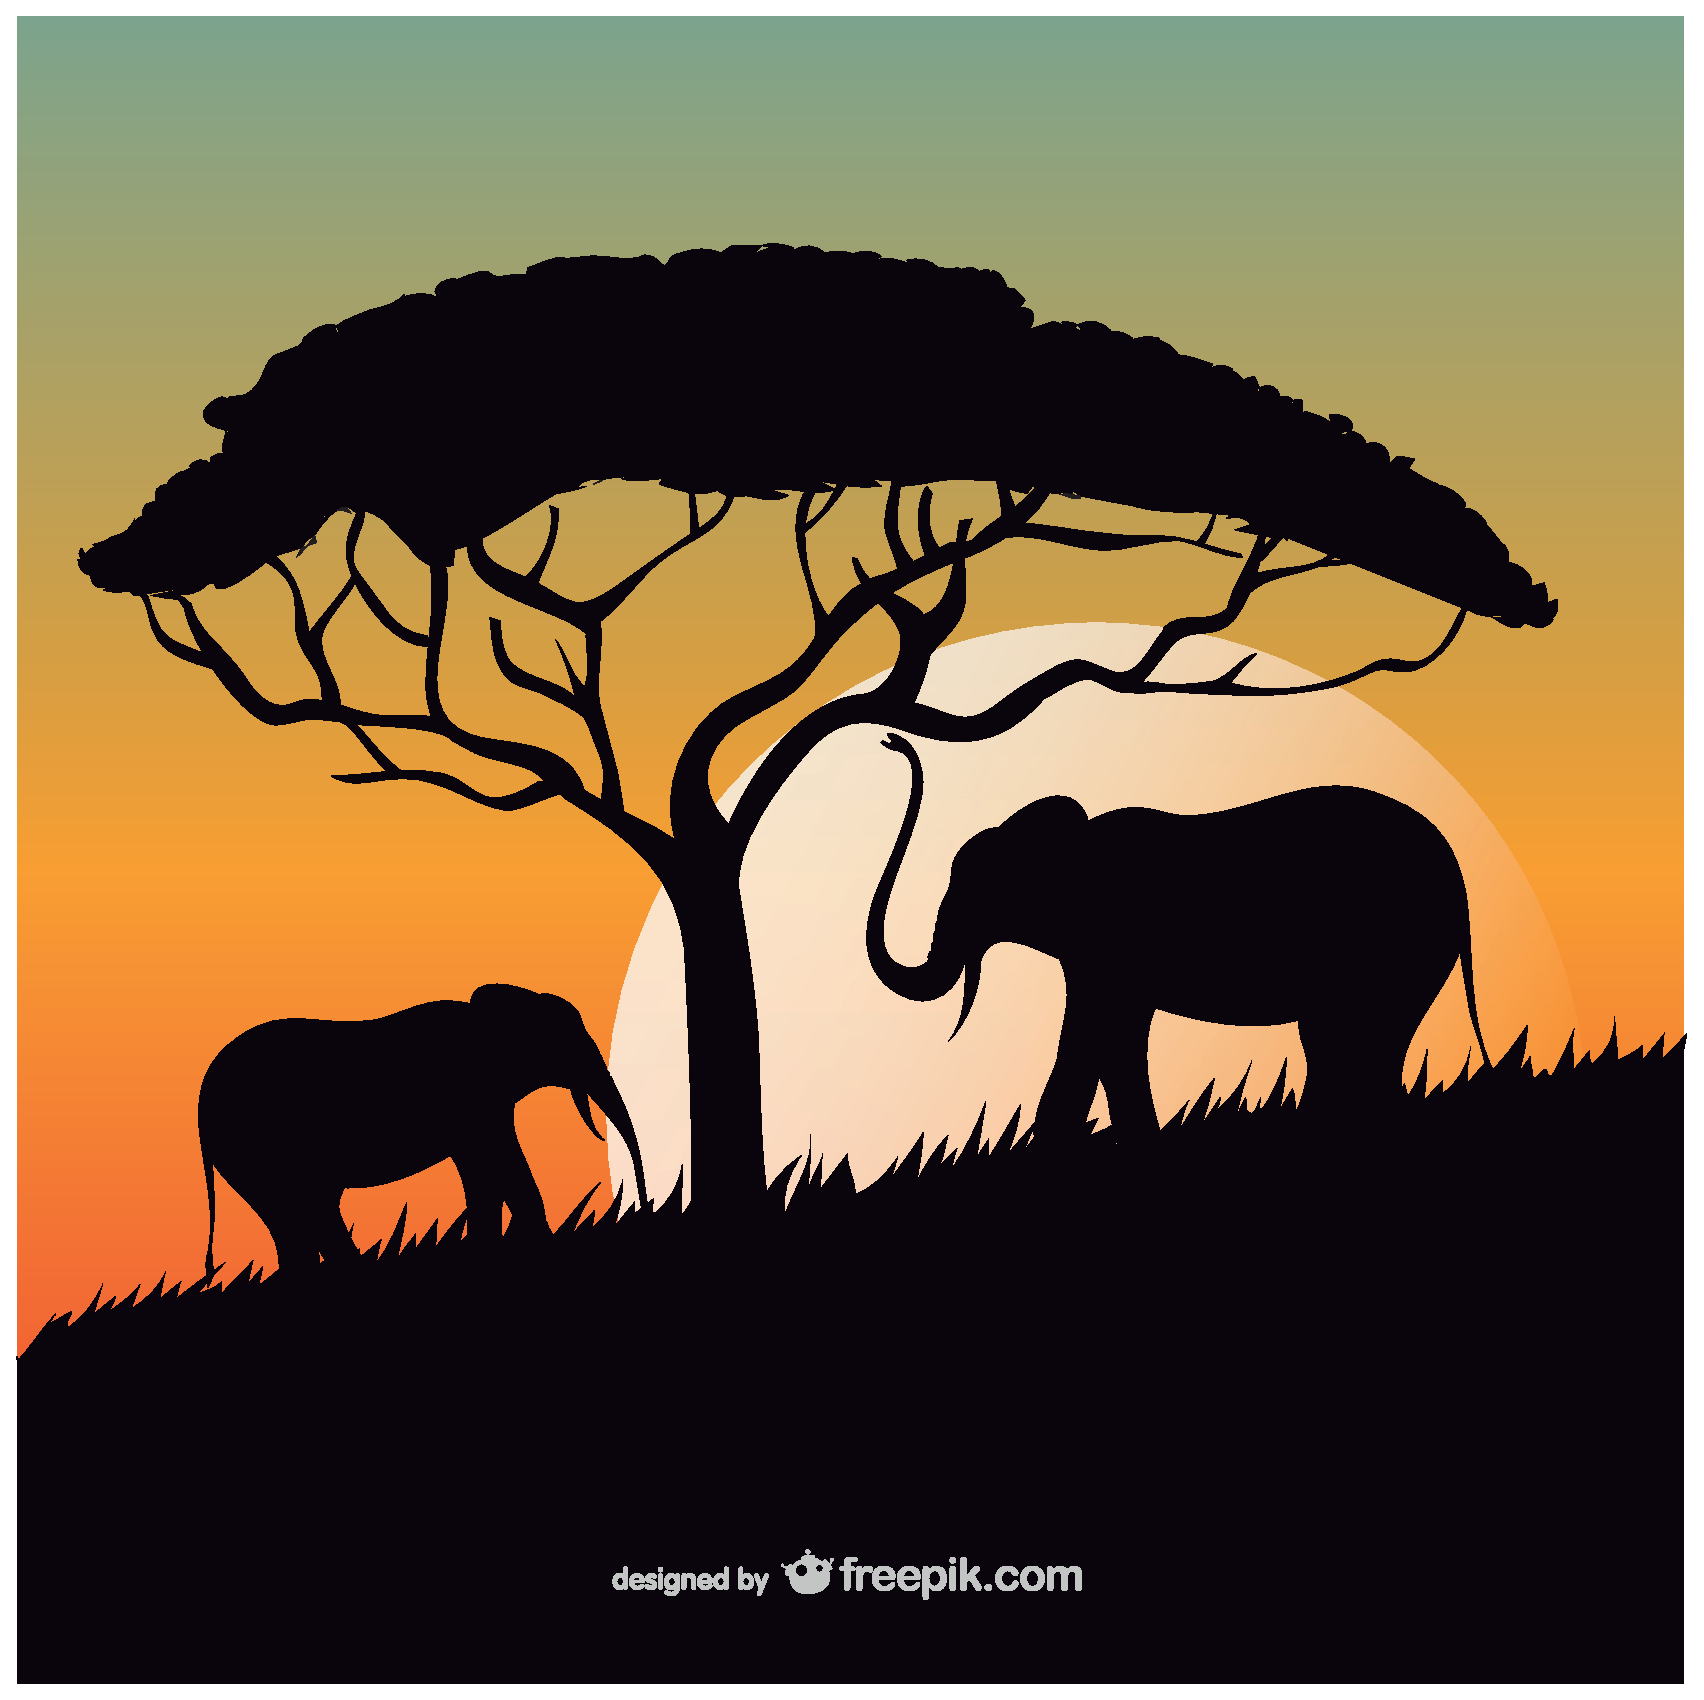
\includegraphics[width=400px, heigh=280px]{683523.eps}
\caption{683523}\label{fig:afryka}
\end{figure}
Na rysunku jest słon \ref {fig:afryka}




\end{document}

